\documentclass[a4paper ,12pt,french]{article}
% Packages usuels
%\usepackage{etex} % pour circuitikz
%\usepackage{tikz}
%\usepackage{circuitikz} % pour les circuits électriques

\usepackage[utf8]{inputenc}
%\usepackage[margin=1.55cm]{geometry}
\usepackage[bottom=2cm , left=2.5cm ,right=2.5cm, top=2cm]{geometry}
\usepackage[T1]{fontenc}
\usepackage{url}
%\usepackage{color}
\usepackage{lmodern}
\usepackage[french]{babel}
\usepackage[indentfirst]{titlesec}
\usepackage[dvips]{graphicx}
\usepackage{eurosym}
\usepackage{amsmath}
\usepackage{amsfonts}
\usepackage{amssymb}
\usepackage{makeidx}
\usepackage{array}
\usepackage{colortbl}
\usepackage[table,dvipsnames,svgnames]{xcolor}
\usepackage{xspace}
\usepackage{fancybox}
\usepackage{textcomp}
\usepackage{listings}


\usepackage{hyperref}
\usepackage{setspace}
\usepackage{fancyhdr}
\usepackage{graphicx}

%\usepackage[margin=0.75in]{geometry}
\usepackage[version=3]{mhchem}
%\usepackage{chemist}
\usepackage{multicol}
\usepackage{float}
\usepackage{wrapfig} %écrire txt et image côte à côte
\usepackage[rightcaption]{sidecap}
\usepackage{amsthm}
\usepackage[squaren, Gray, cdot]{SIunits}
\usepackage[absolute]{textpos}%positionnement de cadres
\usepackage[final]{pdfpages} %traitement des pdf
\usepackage{subfigure}
%\usepackage[framed,numbered,autolinebreaks,useliterate]{mcode}%pour traiter le code matlab
%\usepackage{setspace}% pour les interlignes
%\onehalfspacing %interligne 1.5
%\doublespacing %interligne 2
%\renewcommand{\baselinestretch}{1.5}  %interligne défini
%\usepackage{vmargin}% pour les marges
%\setmarginsrb{2.5}{2.5}{2.5}{2.5}{}{}{}{} % marges de 2.5 cm 
%\addto\captionsfrench{\def\tablename{Tableau}} % pour avoir TABLEAU et pas TABLE dans la légende des tableaux..
%\setlength{\parskip}{1cm}   %espacement fixe entre chaque paragraphe
\setlength{\parindent}{1cm}  %modifie la valeur de l'alinéas
%\addtolength{\voffset}{-1.5cm} % (diminue la marge du haut)
\addtolength{\textheight}{-2cm} % (augmente la longueur du texte)
%\addtolength{\hoffset}{-1cm} (diminue la marge de gauche)
%\addtolength{\textwidth}{2cm}  (augmente la largeur du texte)
%\addtocounter{secnumdepth}{1}  si jamais on veut utiliser \subsubsubsecion
\usepackage[hang,center,bf]{caption} %pour les légendes
\setlength{\captionmargin}{30pt}
\usepackage[hang,flushmargin]{footmisc} %à mettre avec ENGLISH dans babel pour avoir les notes de bas de page à gauche et non indentées
\usepackage[nonumberlist,style=altlist,toc]{glossaries} % Pour faire un glossaire
\makeglossaries
%\addto\captionsfrench{\renewcommand*{\glossaryname}{Glossary}}
\usepackage{wasysym}
\usepackage[square, numbers, comma, sort&compress]{natbib} % Use the natbib reference package - read up on this to edit the reference style; if you want text (e.g. Smith et al., 2012) for the in-text references (instead of numbers), remove 'numbers' 
%\hypersetup{urlcolor=blue, colorlinks=true} % Colors hyperlinks in blue - change to black if annoying
\title{Project 2 - Constraint Programming } % Defines the thesis title - don't touch this
%-------------------------------------------------------------------------------------------------------------------------------------------------------------




\begin{document}

\definecolor{dkgreen}{rgb}{0,0.6,0}
\definecolor{gray}{rgb}{0.5,0.5,0.5}
\definecolor{mauve}{rgb}{0.58,0,0.82}

\lstset{ %
  language=c,                				% the language of the code
  basicstyle=\footnotesize,           	% the size of the fonts that are used for the code
  numbers=left,                   			% where to put the line-numbers
  numberstyle=\tiny\color{gray},  	% the style that is used for the line-numbers
  stepnumber=1,                   			% the step between two line-numbers. If it's 1, each line 
                                  						% will be numbered
  numbersep=5pt,                  			% how far the line-numbers are from the code
  backgroundcolor=\color{white},   % choose the background color. You must add \usepackage{color}
  showspaces=false,               % show spaces adding particular underscores
  showstringspaces=false,         % underline spaces within strings
  showtabs=false,                 % show tabs within strings adding particular underscores
  frame=single,                   % adds a frame around the code
  rulecolor=\color{black},        % if not set, the frame-color may be changed on line-breaks within not-black text (e.g. commens (green here))
  tabsize=4,                      % sets default tabsize to 2 spaces
  captionpos=b,                   % sets the caption-position to bottom
  breaklines=true,                % sets automatic line breaking
  breakatwhitespace=false,        % sets if automatic breaks should only happen at whitespace
  title=\lstname,                   % show the filename of files included with \lstinputlisting;
                                  % also try caption instead of title
  keywordstyle=\color{blue},          % keyword style
  commentstyle=\color{dkgreen},       % comment style
  stringstyle=\color{mauve},         % string literal style
  escapeinside={\%*}{*)},            % if you want to add LaTeX within your code
  morekeywords={*,...}               % if you want to add more keywords to the set
}

\floatstyle{plain}
%\newfloat{graphique}{!hb}{lgr}[chapter]
\floatname{graphique}{Graph}

%\setstretch{1.1} % Line spacing of 1.3

% Define the page headers using the FancyHdr package and set up for one-sided printing
\fancyhead{} % Clears all page headers and footers
\rhead{\thepage} % Sets the right side header to show the page number
\lhead{} % Clears the left side page header

\pagestyle{fancy} % Finally, use the "fancy" page style to implement the FancyHdr headers

\newcommand{\HRule}{\rule{\linewidth}{0.5mm}} % New command to make the lines in the title page

\begin{titlepage}
\pagestyle{fancy} % Finally, use the "fancy" page style to implement the FancyHdr headers

\begin{tabular}{cc}
\begin{minipage}{0.5\textwidth}
\begin{flushleft}

\includegraphics[scale=0.1]{./logoingisbleu.jpg} % University/department logo - uncomment to place it
\end{flushleft}
\end{minipage}
 & 
 \begin{minipage}{0.43\textwidth}
\begin{flushright}

\includegraphics[scale=0.5]{./epl.jpg} % University/department logo - uncomment to place it
\end{flushright}
\end{minipage}
\end{tabular} 



\begin{center}
\vspace{100 px}
\textsc{\LARGE Université Catholique de Louvain}\\[1cm] % University name
\textsc{\Large LINGI2172 - Databases}\\[0.5cm] % Thesis type
 
\HRule \\[0.4cm] % Horizontal line
{\huge \bfseries Mission 3 - Database Design}\\[0.4cm] % Thesis title
\HRule \\[1.5cm] % Horizontal line
 

\begin{tabular}{cc}
\begin{minipage}{0.5\textwidth}
\begin{flushleft} \large
\emph{Authors:}\\
{Baugnies Benjamin (6020-10-00)\\
Colson Olivier (5039-10-00)\\
Vanwelde Romain (3143-10-00)\\ \ \\Group 3} 
\end{flushleft}
\end{minipage} & \begin{minipage}{0.46\textwidth}
\centering
\begin{flushright} \large
\emph{Supervisers:} \\
{Pr. Bernard Lambeau\\
Antoine Cailliau\\
}
\end{flushright}
\end{minipage}\\[3cm] \\ 
\end{tabular} 

 
%\large \textit{A thesis submitted in fulfilment of the requirements\\ for the degree of \degreename}\\[0.3cm] % University requirement text
%\textit{in the}\\[0.4cm]
%\groupname\\\deptname\\[2cm] % Research group name and department name

 \begin{center}
{\large \today }\\[4cm] % Date 
 \end{center}


\vfill
\end{center}

\end{titlepage}

\lhead{\emph{Databases}} % Set the left side page header to "Contents"
%\tableofcontents % Write out the Table of Contents

\thispagestyle{fancy}

\pagebreak
\setcounter{page}{1}
\pagestyle{fancy} % Finally, use the "fancy" page style to implement the FancyHdr headers
\section{Introduction}

Telling a story is challenging. Indeed, in order to build a ``good" scenario, one must think of a lot of different aspects and ensure coherence between all these points. \\

Some can manage it using diagrams, other can rely on tons of paper sheets referencing each other or, more reasonably, use a computer to store all their documents. However, with all these ways of working, the same problem arises: as the storyline and background get denser, it becomes more and more difficult to ensure that no contradiction appears. This is a big problem, since contradictions ruin the feeling of reality that must always be given by a good scenario. How about asking the computer to gather, interpret and display all this information in a clean and understandable way?\\

Our project can be defined as a ``narration manager". Its goal is to make it easier for people to write coherent and complex scenarios without either becoming mad or cancelling their project because of its increasing complexity. It is intended for all "story makers" (videogame makers, film makers, roleplayers, writers, \dots), and is thus meant to be generic and conveniently adapt to various situations, as well as user preferences and priorities in the story (for example, some users could want to define a precise date for each event happening in their story, as others could prefer to focus on the relations binding all the characters together).\\

Possibilities of telling a story are infinite, yet time and coordination constraints often limit what is actually possible to achieve. It is now time to push these limits away.
 
\section{Elementary Facts}

Bellow are some elementary facts we wrote to better understand what to do, which relation exists between all the entities.

\subsection{About characters}

\noindent Pierre is from Bruxelles.\\
Pierre is born on 28/12/1992\\
Jean is born on 01/04/1992\\
Benjamin is born on 03/06/1992\\
Jean is melancholic\\
Benjamin is member of the association "Les Petits Riens"

\subsection{Characters relations}
\noindent Pierre liked Benjamin from 9/12/2002 to 13/7/2007.\\
Benjamin liked Pierre from 10/11/2003 to 12/8/2009.\\
Jean doesn't like Benjamin from 10/11/2003 to 12/8/2009.\\
Paul is Pierre's father.\\
Pierre is Paul's son since 28/12/1992.\\


\subsection{About events}

\noindent Jean attended the event "The beer festival"\\
The "beer festival" took place at LLN\\
The "beer festival" lasted from 08/03/2014 to 18/03/2014.\\
The "beer festival" is "blablablablablablablabla" as description.


\subsection{About places}
\noindent Intel room is a sub-location of Réaumur's Map and is represented on square number 10.\\
Réaumur is a sub-location of  LLN's Map and is represented on square number  5.\\
The LLN's Map represents the location "LLN"\\
The Réaumur's Map represents the location "Réaumur"\\
LLNMap has 10 square width, and represents a 5km distance.\\
LLNMAP has 20 square length, and represents a 10km distance.

\section{ORM schema}


The ORM schema is shown on the Figure \ref{orm}. If some relations are too difficult to read, the numeric version is available in the Annexes directory of the zip file.\\
\begin{figure}[!h]
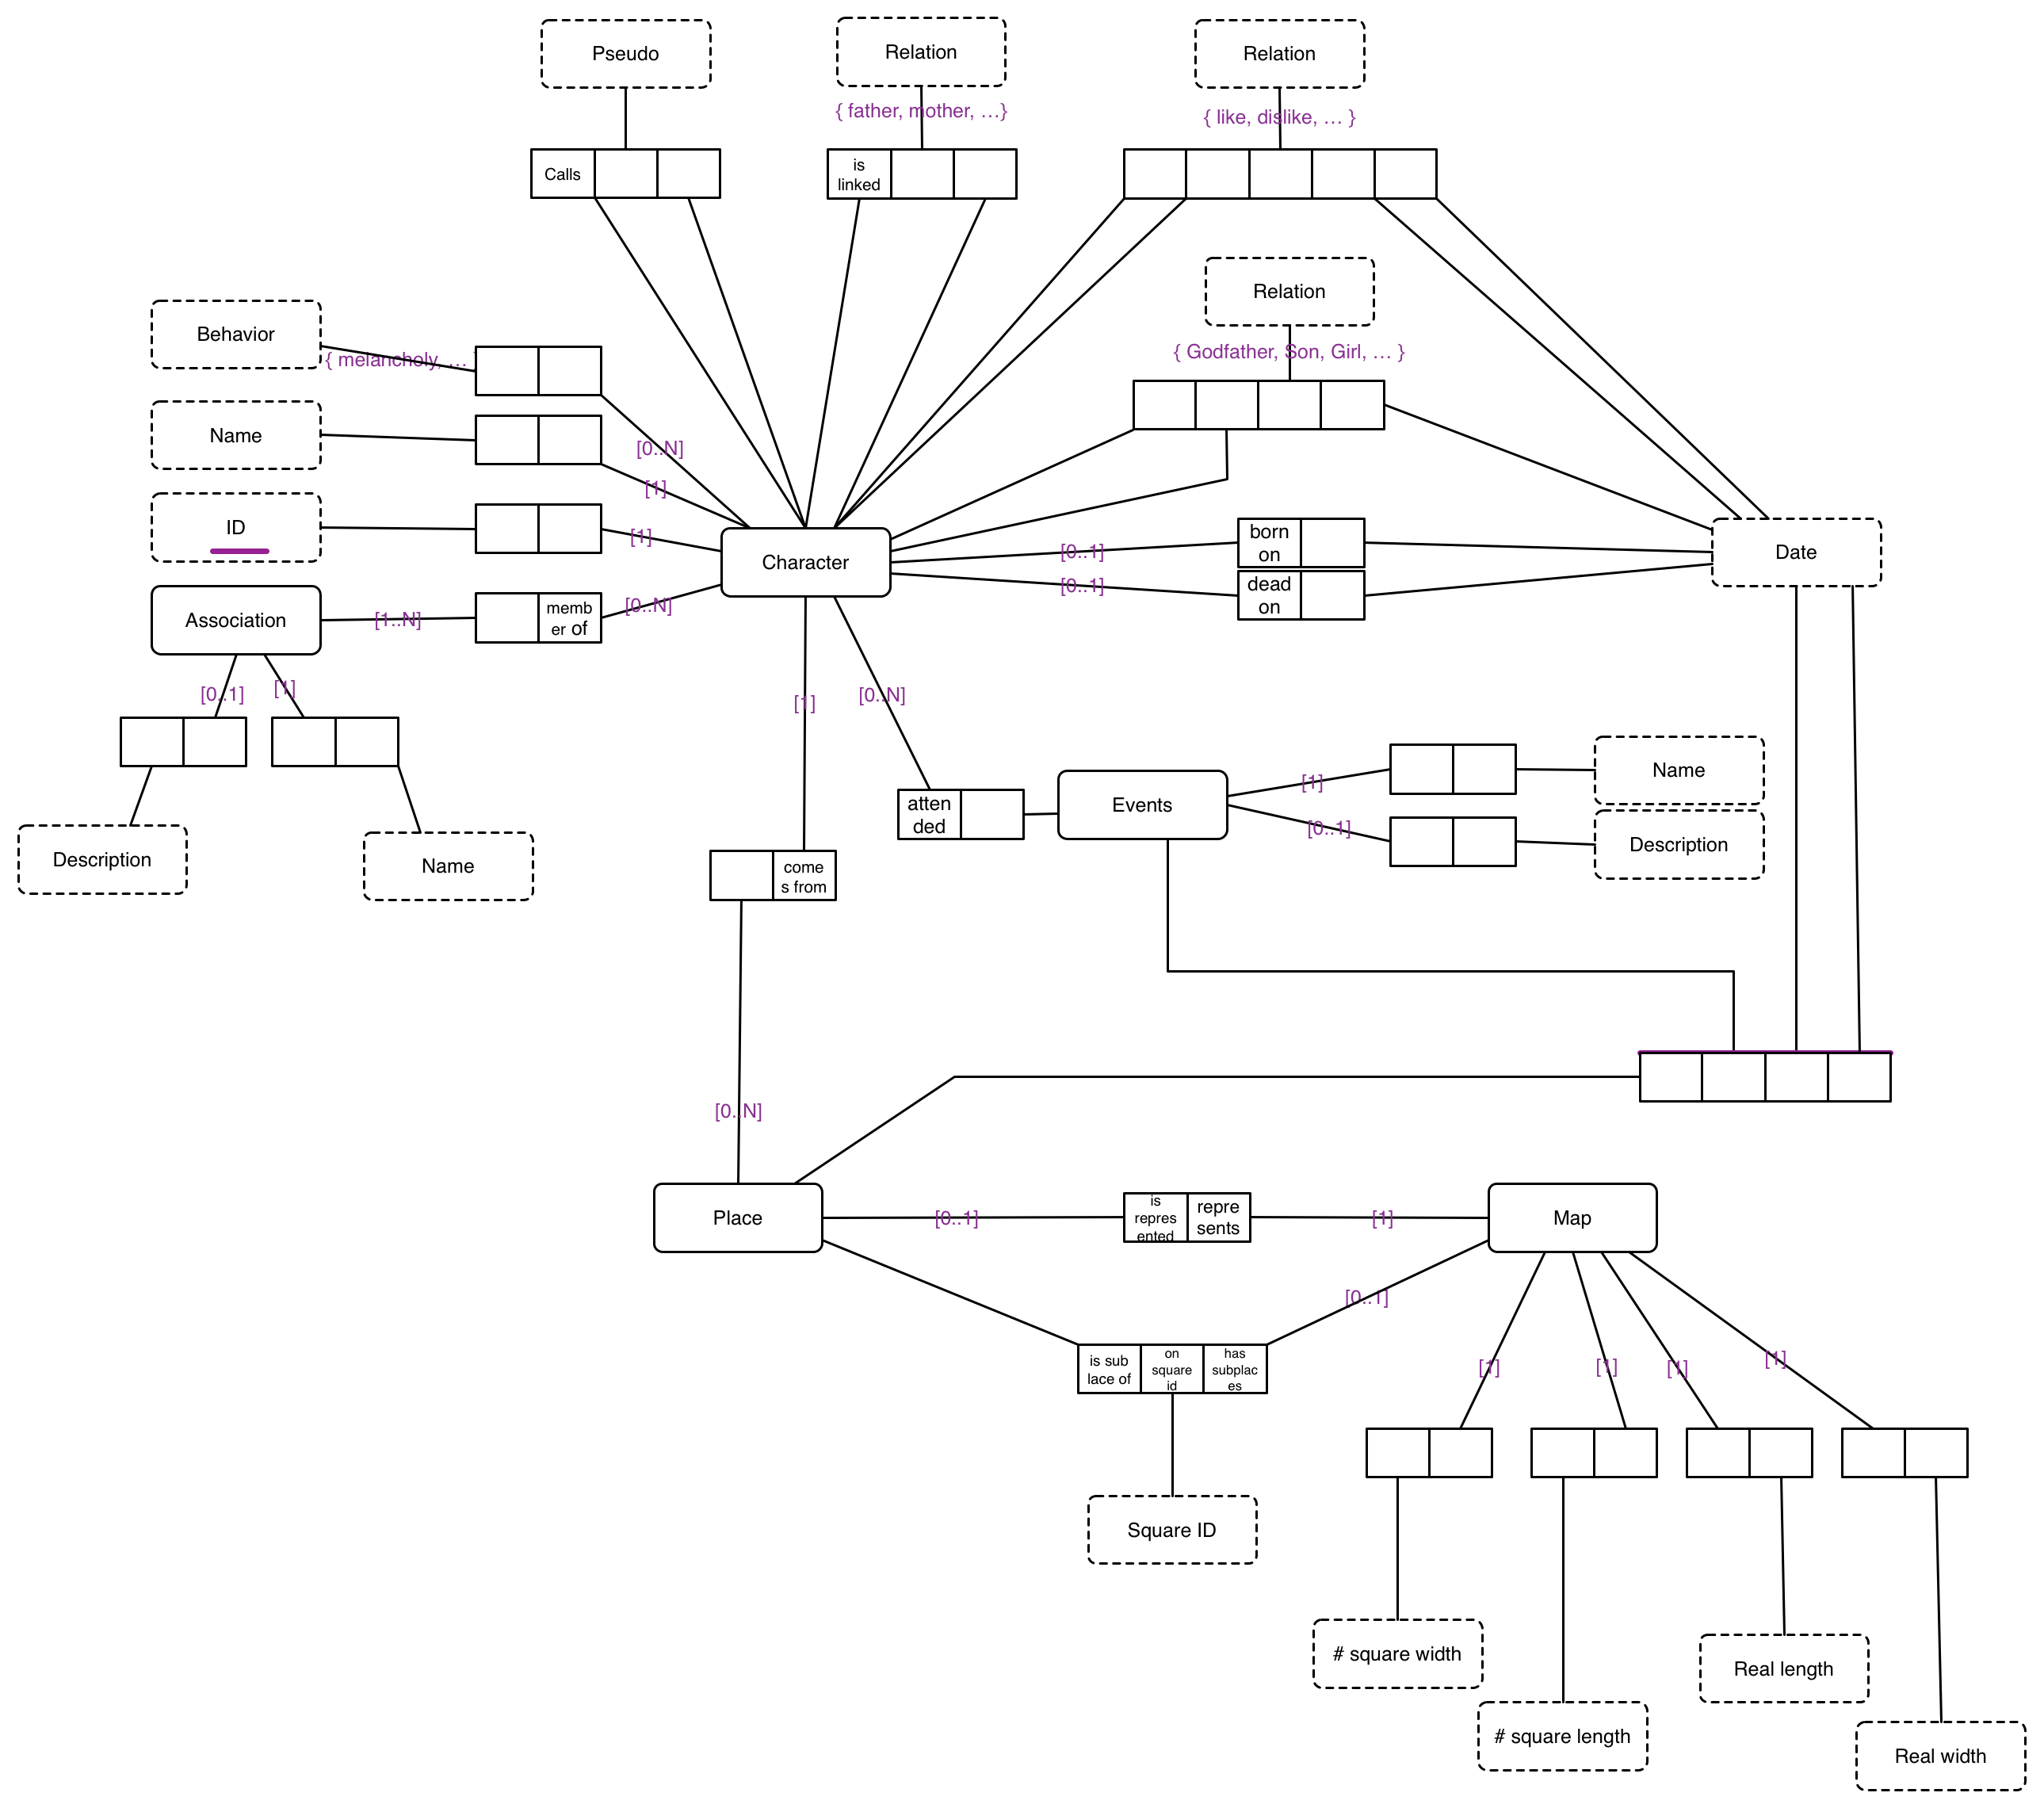
\includegraphics[scale=0.43]{ORM.png}
\caption{ORM Schema}
\label{orm}
\end{figure}

As we can see on the schema, there are 4 main entities which are \texttt{"Characters''}, \texttt{"Events''}, \texttt{"Place''}, and \texttt{"Map''}.


We will explain here above three specific case of the diagram :\\

\textbf{Character - Relation relations involving time range, time or timeless notion.} \\
The relations explain the relationships between different characters. They are uni-directional and the different kinds of relations can be defined by the user.
We split these relations into three types to represent the fact that some relations are time-independent (e.g "\dots is my father"), some can start at a given time and be permanent and/or open-ended (e.g "\dots is my godfather since \dots"), and finally some can last for only a while (e.g "\dots was my friend from \dots to \dots").\\

\textbf{Pseudo relation.} \\
This relation involves two characters and a pseudonym. It describes the name used by the first character for the second one. This represents the fact that during the story, a given character might not know another's real name. We added this relation since this can have an impact on the story (he wouldn't realize others were talking about someone he knows for example).
The corresponding table will also allow us the find all the pseudonyms a given person might go by.\\

\textbf{Place - Map relation.} \\
This is a rather complex relation that we introduced to keep track of a story's geography at different levels. The first use is to allow users to situate events or characters. We can also define sub-places to refine locations. 
We can see that a place's map is optional. However, since a place's sub-places are linked to its map, it implicitly  becomes required when we want to add levels. This structure allows us to chain an arbitrary number of levels with a "place - map - place - map - \dots" hierarchy.
This relation has two constraints that are not expressed in the database and will have to be verified in the software implementation. Firstly, the map square on which the sub-place is located must belong to the map's domain of possible squares (between 1 and (\# square width)*(\# square length)). Secondly, it is required that two places of the same level do not overlap.

\section{Tutorial-D script}

In the zip file, you can find files \texttt{structure\_rel.d} and \texttt{data\_rel.d}.\\

\textbf{structure\_rel.d} has three differents parts. The \textbf{first} one is the definition of special types (All the entities ID, and one for some names too). Then, the \textbf{second} part is all the relvars, with all primary keys, and also unique keys (e.g. \texttt{MAPPEDPLACE} which has one key on the PLACEID and another on the MAPID). The third part is all the constraints which are foreign keys. We express first all the constraints implying CHARID, then implying ASSOCIATIONID, and so on.\\

\textbf{data\_rel.d} fills the database with all elementary facts expressed before in the report.

\section{Relvar predicates}
In this section, we will give the relvar predicates that our database represents. The attributes of a relation are in bold, and the attributes that form the key are underlined.

\subsection*{About characters:}
\begin{itemize}
\item The character \underline{\textbf{CHARACTERID}} is named \textbf{NAME}. \underline{\textbf{ASSOCIATIONID}}.
\item The character \underline{\textbf{CHARACTERID}} has a behavior that is \underline{\textbf{BEHAVIOR}}.
\item The character \underline{\textbf{CALLERID}} knows the charactert \underline{\textbf{CALLEID}} by the pseudonym \underline{\textbf{PSEUDONYME}}.
\end{itemize}

\subsection*{About time:}
\begin{itemize}
\item The character \underline{\textbf{CHARACTERID}} was born on \textbf{BIRTH}.
\item The character \underline{\textbf{CHARACTERID}} died on \textbf{DEATH}.
\end{itemize}

\subsection*{About Associations:}
\begin{itemize}
\item The association \underline{\textbf{ASSOCIATIONID}} is named \textbf{NAME}.
\item The association \underline{\textbf{ASSOCIATIONID}} is described as \textbf{DESCRIPTION}.
\item The character \underline{\textbf{CHARACTERID}} is a member of the association.
\end{itemize}

\subsection*{About character relations:}
\begin{itemize}
\item The relation \underline{\textbf{RELATIONID}} is of the type \textbf{RELATIONSHIP}.
\item The character \underline{\textbf{SOURCE}} has a timeless relation with \underline{\textbf{TARGET}} of the type \underline{\textbf{RELATIONID}}.
\item The character \underline{\textbf{SOURCE}} started a permanent relation with \underline{\textbf{TARGET}} of the type \underline{\textbf{RELATIONID}} at the time \underline{\textbf{DATE}}.
\item The character \underline{\textbf{SOURCE}} had a relation with \underline{\textbf{TARGET}} of the type \underline{\textbf{RELATIONID}} that started on \underline{\textbf{START}} and ended on \underline{\textbf{ENDDATE}}.
\end{itemize}

\subsection*{About places:}
\begin{itemize}
\item The place \underline{\textbf{PLACEID}} is called \textbf{PLACENAME}.
\item The map \underline{\textbf{MAPID}} has a width of \textbf{WIDTH} split into \textbf{NUMWIDTH} sections, and a length \textbf{LENGHT} split into \textbf{NUMLENGTH} sections.
\item The place \textbf{PLACEID} is represented by the map \underline{\textbf{MAPID}}.
\item The place \underline{\textbf{PLACEID}} is locate on the square \underline{\textbf{SQUAREID}} of the \underline{\textbf{MAPID}} map.
\item The character \underline{\textbf{CHARACTERID}} originates from \textbf{PLACEID}.
\end{itemize}

\subsection*{About events:}
\begin{itemize}
\item The event \underline{\textbf{EVENTID}} is named \textbf{NAME}.
\item The event \underline{\textbf{EVENTID}} is described as \textbf{DESCRIPTION}.
\item The character \underline{\textbf{CHARACTERID}} attended \underline{\textbf{EVENTID}}.
\item The event \underline{\textbf{EVENTID}} happened at \underline{\textbf{PLACEID}}, started on \underline{\textbf{BEGINNING}}, and ended on \underline{\textbf{ENDDATE}}.
\end{itemize}

\section{General Architecture}
Our program uses an Model, View, Controller (MVC) template. 

\subsection{Models}
The model files are classes used to have an in-memory representation of the DB data. Most of our models extend the DBModel abstract class which contains all the mandatory information for every model type, (most notably the ID) and allows certain methods to apply to any type of Model. The exceptions are CharacterPseudoData and RelationData, which do not use IDs. Our current models are:
\begin{itemize}
\item AssociationModel (non implemented)
\item CharacterModel
\item CharacterPseudoData
\item MapModel
\item PlaceModel
\item RelationData
\end{itemize} 
 \paragraph*{} What these classes represent is fairly obvious. It is important to note that the models are strongly connected. Indeed, an event will contain information about the characters that participated. These characters will in turn contain information about the other events they attended. From there, it is not difficult to imagine scenarios where every model is somehow related to every other one, resulting in the whole database being loaded into memory when accessing a single character.
In order to avoid this, a number of models do not contain instances of other models, but references to them (in this case, the String representation of the database ID). For example, a character model contains a LinkedList of the IDs of the events he attended. It is also usefull to note that EditionTableModel is not a model in this context, despite its name. Indeed, it is an implementation of the TableModel interface which is used for building the GUI.\\ \\

\subsection{Views}
The View classes (named Windows in our program) dictate how the models are represented in the GUI. All our Windows are aimed at creating or editing a model while viewing it at the same time. To facilitate this, they extend an abstract EditionWindow class which provides the default methods for building the GUI, as well as the facilities to communicate with the Controller The one exception is MainMenu, which of course does not manipulate any data. The implemented Views are:
\begin{itemize}
\item CharacterEditionWindow
\item EventEditionWindow
\item MainMenu
\item MapChoiceWindow
\item MapCreateWindow
\item PlaceEditionWindow
\item RelationEditionTable
\end{itemize}

\paragraph*{}
In almost every case, the same view is used to both create and update/view a model. The exception is for the map. Indeed, viewing a map involves displaying the Events and subplaces on it, while creating it only involves collecting its dimensions.

\subsection{Controller}
The controller is a single class that acts as a bridge between the Models and Views. Its tasks are to give the Views access to the data from the Models to fill the GUI with the relevant information. It is also in charge of controlling what happens when one View is closed. Depending on what happened, it will launch the next View and/or perform the corresponding database manipulations though not directly, as we will explain in the next part.

\subsection{Other files}
Some files do not belong strictly to the MVC pattern but are used for convenience. The most important of them is the DatabaseCoordinator. This class provides a layer between the Database and the MVC. The main utility of this class is to group all the SQL queries into a single class, in order to abstract away from the SQL language in the rest of the program. \\ \\
The other files are:
\begin{itemize}
\item NarrationManager: acts as Main class, starts the Controller
\item NarrationDate: simple class to represent a date without our calendar's restrictions
\item EditionTableModel: implementation of java AbstractTableModel (which implements TableModel), used for tabular representations in a GUI as a model for JTable.
\item EditionTable: an extension of JTable to provide common functionalities between its different extensions.
\item EditionTablePanel: extension of JPanel to contain an EditionTable and add default buttons (apply and cancel).
\item EventEditionTable/RelationEditionTable: extensions of EditionTable to provide a table layout of the corresponding model.
\end{itemize}


\section{Implementation issues}
Due to various factors, we did not achieve all the things we would have wanted to do. In this section we will go the main features would have liked to add to the program.

\subsection{DB coherence}
Our current implementation uses queries directly through the JDBC driver. However, certain manipulations of the database require queries to multiple tables. I the event that one of the queries is invalid (wrong parameters, system crash ...), the others are not stopped and no recovery system is used. Additionaly, the users is not warned when one or more queries fail. This can result in situations where data might not have been added to the DB while the user thinks it is, or where some of the data is written in the DB while the user thinks the whole modification was dropped.
Given more time, we would have wished to add mechanisms to warn the user in the event that he provided an invalid input before executing the query. Additionaly, we would have modified the project to use transactions to add data to the DB in a safe and reliable way.

\subsection{Design oversights}
When the moment came for us to gather statistics for the user, we realized we had forgottent a simple but important field for characters: their gender. This had the unfortunate consequence of making one of our big objectives (giving the user a quick overview of information over the whole text) a lot more complicated.
We did consider some workaround solutions, such as representing gender by a self to self "Relation" (character relation, not DB relation), but this would cause gender statistics to be indistinguishable from other relations.

\subsection{Missing features}
Many features were not implemented due to the size of the project and the time given. As mentioned in the previous paragraph, statistics on gender were made difficult because of an oversight, and the whole feature  ended up being dropped. We also did not have time to create a satisfactory Place viewer like those for Characters and Events. Ultimately, this viewer would have contained an interactive map representation of the place. This map would would show the Events and Subplaces of the Place, and would change depending on the time.
Another feature that was not implemented is the handling of Character behaviour. This is simply another characteristic of a character, on which statistics would also have been collected. Similarly, Associations were not implemented beyond creating the empty model file.

\section{SQL script}

In the zip file, you can find files \texttt{structure.sql} which builds the entire structure of the database in SQL. This script is idempotent, and is build with the same structure as the tutorial-D script. Indeed, we first create all the tables with the primary keys/unique keys, then we alter them to add the foreign key constraints.\\


The file \texttt{data.sql} is also available in the zip file. This one is also idempotent. It builds the structure of the database as the previous file, then it fills the database with all the elementary facts presented above in the report.
\newpage
\section*{Annexes}
\appendix

\section{Code Rel}
\lstinputlisting[language=java]{structure_rel.d}
\newpage
\section{Code SQL}
\lstinputlisting[language=sql]{structure.sql}



\end{document}